% Created 2021-03-14 Sun 16:03
% Intended LaTeX compiler: pdflatex
\documentclass[11pt]{article}
%% \documentclass[11pt,twocolumn]{article}
\usepackage[utf8]{inputenc}
\usepackage[T1]{fontenc}
\usepackage{graphicx}
\usepackage{grffile}
\usepackage{longtable}
\usepackage{wrapfig}
\usepackage{rotating}
\usepackage[normalem]{ulem}
\usepackage{amsmath}
\usepackage{textcomp}
\usepackage{amssymb}
%% \usepackage{capt-of}
\usepackage{hyperref}
\usepackage{xcolor}
%% \usepackage{underscore}
\usepackage{setspace}
%% \usepackage{verbatimbox}
%% \setlength{\columnsep}{1.9pc}
%% \usepackage[obeyspaces]{url}
\usepackage{caption}
\captionsetup{font=small,labelfont=bf}
\usepackage{multicol}
%% \setlength\columnseprule{.4pt}


%% \setlength{\columnseprule}{1pt}
%% \def\columnseprulecolor{\color{blue}}

\date{\today}
\title{Entropy in Evolutionary Algorithms}
\author{Lucas Blakeslee\footnote{\texttt{lqblakeslee@gmail.com}},
  Aengus McGuinness\footnote{\texttt{aengus82520@gmail.com}}}
\hypersetup{
 pdfauthor={},
 pdftitle={},
 pdfkeywords={},
 pdfsubject={},
 pdfcreator={Emacs 27.1 (Org mode 9.3)}, 
 pdflang={English}}

\setlength\parindent{24pt}

\begin{document}
\maketitle
%% \tableofcontents


\label{sec:org26f53e0}
\begin{abstract}
\label{sec:orga17da23}
Genetic algorithms (GAs) are an optimization technique inspired by
natural selection. GAs have yielded good results in certain practical
problems, yet there is still more to be understood about their
behavior on a theoretical level. One approach is to look at the
evolutionary process from the point of view of statistical mechanics,
and interpreting jumps in fitness as phase transitions. Toward this
goal we examine the behavior of \emph{entropy} in a GA that optimizes
a simple function.  We find that entropy increases as a new species
diversifies, but its upper bound decreases with most phase
transitions (which correspond to evolutionary steps).
\end{abstract}


%% -\textbf{- mode: org -}-


\section{Motivation}
\label{sec:org16abecd}
Genetic algorithms (GAs) are stochastic search algorithms based on the
process of natural evolution, solving for the 'fittest' solutions to a
problem. GAs are optimization algorithms, designed to maximize or
minimize certain functions. GAs are much more efficient than random or
exhaustive search algorithms (Kinnear, 1994), however, they do not
scale well with complexity (Radcliffe \& Surry, 1995). While specifics
may vary, there are some processes universal to GAs, which are:
population → fitness evaluation → selection → crossover → mutation,
repeat. Each organism in the population has its own 'chromosome,' or
set of characteristics. Here is where the resemblance to biological
evolution begins to weaken. GAs continue to occur either
until some condition for termination has been met, or until a
pre-specified number of iterations has elapsed. \\
Genetic algorithms
have been used in a variety of practical applications, from making
"evolved antennae" for spacecrafts and satellites to the estimation of
heat flux between sea ice and the atmosphere to predictive economic
models. \\
Entropy and evolution have been often explored together, with
research on the subject going as far back as the 1870s, though
Schrödinger's 1944 book \emph{What is life?} sparked a wave of modern
interest. Here we wondered how entropy would change over time in a
genetic algorithm, in order to attain a better theoretical grasp of
how they function.

\section{Hypothesis}
\label{sec:org26a3be1}
We hypothesized that entropy would gradually rise as small
non-significant mutations occured, and that occasionally one highly
beneficial mutation in an organism would cause entropy to rapidly
decrease as that mutation was selected for and spreads throughout the
population, and that entropy would then begin to rise again in a
cyclical pattern. We hypothesized that if we're considering entropy to
be the number of possible states an organism can be in, the upper
bounds of the entropy would never reach levels they were previously
at.


\section{Genetic algorithms in Brief}

In brief Genetic Algorithms attempt to find the maximum value of a
function (called a \emph{fitness} function), such as those shown in
Figure~\ref{fig:fit-func_pid3095791}

They do so by having a population of candidate values that take steps
through the domain of that function.  The steps have a random
component, but the randomness is directed by a principle akin to
natural selection: when a population member has a high fitness value,
it is more likely to survive and breed new population members that
share some of its characteristics.

Figure~\ref{fig:gen-info_pid3095791} shows an example of such an
evolution.

Some terminology is used in talking about GA evolution:

\begin{description}
\item[Population] The collection of values currently being considered
  as possible solutions to the problem.
\item[Fitness] A function for which we are trying to find the maximum.
\item[Fitness Landscape] A visualization of the fitness function which
  shows the peaks in fitness, as well as the pitfalls in searching for
  the peaks.
\item[Reproduction] The breeding of two parent individuals into two
  children. Organisms are floats, and we can think of them as
  sequences of 32 bits in IEEE 754 format.
\item[Mutation] At the end of each generation the organisms undergo
  "mate drift" mutation, wherein their offspring shift a small amount
  in one direction, with a low possibility of large drifts occuring.
\end{description}



\section{Approach}
\label{sec:org8c588e5}

To explore how the entropy of the GA population behaves we crafted an
optimization problem that would bring out some well defined steps in
fitness improvement, and also allow a period of stasis between
successive fitness peaks.

\subsection{Fitness functions}

The function we settled on is shown in
Figure~\ref{fig:fit-func_pid3095791}: peaks are separated by valleys,
and it can take the evolutionary process a while for a mutation to
transport a population member across the valley and into the higher
fitness area.

\begin{figure}
  \centering
  \resizebox{\linewidth}{!}{%
  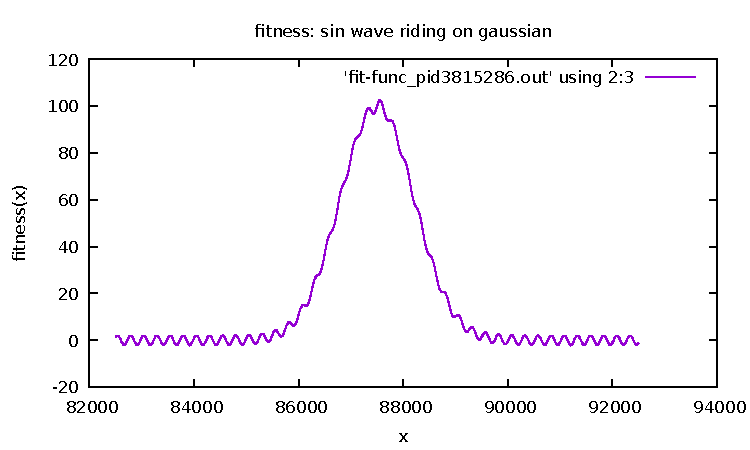
\includegraphics{fit-func_pid3815286.pdf}
  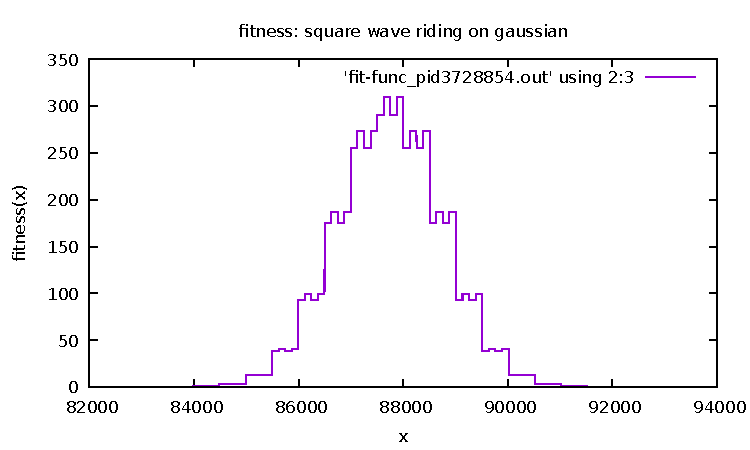
\includegraphics{fit-func_pid3728854.pdf}
  }
  \caption{Two examples of fitness functions: one has a $\sin()$ wave
    riding on a gaussian, the other has a flat-top wave riding on it.
  Most of our results are based on the ``flat-top'' function.}
  \label{fig:fit-func_pid3095791}
\end{figure}

In addition to these two fitness functions, we have also used a
polynomial fitness function, where the GA searched for the highest
peak in a negative degree polynomial. However, we found that the
polynomial fitness function was not rich enough to yield interesting
results.



\subsection{Shannon Entropy}

At each step in the evolution we calculate the \emph{Shannon Entropy},
a measure of the information content by applying Shannon's formula to
the population $P$:
\begin{equation}
H({\rm P}) = -\sum_{x \in {\rm P}} p(x)\log p(x)
\label{eq:shannon-entropy-def}
\end{equation}
where $p(x)$ is the probability that a member of the population be in
\emph{state} $x$.  When our population consists of values on the real
number line, our state will be a narrow band of numbers.  In other
types of population (such as animal populations) the state could mean
something else, like eye color, or number of fingers, or ability to
walk upright.

Shannon Entropy is widely discussed elsewhere, but we can mention that
the entropy relates to the \emph{disorder} or \emph{randomness} in the
population.\footnote{Equating entropy to disorder is not the most
rigorous definition, but it is good enough for our purposes here.}

We can also give a simple example here.  Let us look at words of text
in a paragraph.  The ``population'' are the words (a sequence of
characters separated by spaces).

We will examine four different paragraphs that we have contrived: one
which just repeats a single word, the other repeats a sequence of two
words, the third has English text with some repetitions (in fact we
repeat the whole phrase a few times), and the fourth is a bunch of
random strings of letters broken up in to words.

%% \begin{multicols}{2}


\subsubsection{single word}

\begin{tiny}
\begin{verbatim}
==================== one_word_para =======================
dude dude dude dude dude dude dude dude dude dude dude dude dude dude
dude dude dude dude dude dude dude dude dude dude dude dude dude dude
dude dude dude dude dude dude dude dude dude dude dude dude dude dude
dude dude dude dude dude dude dude dude dude dude dude dude dude dude
dude dude dude dude dude dude dude dude dude dude dude dude dude dude
dude dude dude dude dude dude dude dude dude dude dude dude dude dude
dude dude dude dude dude dude dude dude dude dude dude dude dude dude
dude dude dude dude dude dude dude dude dude dude dude dude dude dude
dude dude dude dude dude dude dude dude dude dude dude dude dude dude
dude dude dude dude dude dude dude dude dude dude dude dude dude dude
dude dude dude dude dude dude dude dude dude dude dude dude dude dude
dude dude dude dude dude dude dude dude dude dude dude dude dude dude
dude dude dude dude dude dude dude dude dude dude dude dude dude dude
dude dude dude dude dude dude dude dude dude dude dude dude dude dude
dude dude dude dude dude dude dude dude dude dude dude dude dude dude
dude dude dude dude dude dude dude dude dude dude dude dude dude dude
dude dude dude dude dude dude dude dude dude dude dude dude dude dude
dude dude dude dude dude dude dude dude dude dude dude dude dude dude
dude dude dude dude dude dude dude dude dude dude dude dude dude dude
dude dude dude dude dude dude dude dude dude dude dude dude dude dude
dude dude dude dude
=================== end of one_word_para ==================
\end{verbatim}
\end{tiny}

In this example the only word that ever comes up is the word
\texttt{``dude''}, and its probability is $p({\rm dude}) = 1$.  Using
this in Shannon's formula, together with the fact that
$$lim_{x\rightarrow 1}x \log(x) = 0$$
we get $H = 0$.

So if all members of the population are identical, then the Shannon
entropy is zero.

\subsubsection{two word sequence}


%% \end{multicols}

\begin{tiny}
\begin{verbatim}
==================== two_word_para =======================
two dudes two dudes two dudes two dudes two dudes two dudes two dudes
two dudes two dudes two dudes two dudes two dudes two dudes two dudes
two dudes two dudes two dudes two dudes two dudes two dudes two dudes
two dudes two dudes two dudes two dudes two dudes two dudes two dudes
two dudes two dudes two dudes two dudes two dudes two dudes two dudes
two dudes two dudes two dudes two dudes two dudes two dudes two dudes
two dudes two dudes two dudes two dudes two dudes two dudes two dudes
two dudes two dudes two dudes two dudes two dudes two dudes two dudes
two dudes two dudes two dudes two dudes two dudes two dudes two dudes
two dudes two dudes two dudes two dudes two dudes two dudes two dudes
two dudes two dudes two dudes two dudes two dudes two dudes two dudes
two dudes two dudes two dudes two dudes two dudes two dudes two dudes
two dudes two dudes two dudes two dudes two dudes two dudes two dudes
two dudes two dudes two dudes two dudes two dudes two dudes two dudes
two dudes two dudes two dudes two dudes two dudes two dudes two dudes
two dudes two dudes two dudes two dudes two dudes two dudes two dudes
two dudes two dudes two dudes two dudes two dudes two dudes two dudes
two dudes two dudes two dudes two dudes two dudes two dudes two dudes
two dudes two dudes two dudes two dudes two dudes two dudes two dudes
two dudes two dudes two dudes two dudes two dudes two dudes two dudes
=================== end of two_word_para ==================
\end{verbatim}
\end{tiny}

In this example there are only two words: \texttt{``dudes''} and
\texttt{``two''}.  Each occurs 140 times, for a total of 280 words.

There are only two probabilities to calculate: $p({\rm two}) = 1/2$
and $p({\rm dudes}) = 1/2$.

So the Shannon formlula (Equation~\ref{eq:shannon-entropy-def}) gives
us:
$$
H({\rm P}) = -\frac{1}{2}\log\frac{1}{2} - \frac{1}{2}\log\frac{1}{2}
= 0.693
$$

So with exactly two possible states, and the population divided
equally between them, the entropy is $0.693$.


\subsubsection{English paragraph}

\begin{tiny}
\begin{verbatim}
==================== english_para =======================
This is a simple paragraph of English text We hope that there will be
many words that occur repeatedly.  The English language has many words
and this paragraph might have many repetitions.  The hope is that there
are enough repetitions.  So I ask: will the entropy be big or small?
The answer is that we will have to see what the program returns. This is
a simple paragraph of English text We hope that there will be many words
that occur repeatedly.  The English language has many words and this
paragraph might have many repetitions.  The hope is that there are
enough repetitions.  So I ask: will the entropy be big or small?  The
answer is that we will have to see what the program returns. This is a
simple paragraph of English text We hope that there will be many words
that occur repeatedly.  The English language has many words and this
paragraph might have many repetitions.  The hope is that there are
enough repetitions.  So I ask: will the entropy be big or small?  The
answer is that we will have to see what the program returns. This is a
simple paragraph of English text We hope that there will be many words
that occur repeatedly.  The English language has many words and this
paragraph might have many repetitions.  The hope is that there are
enough repetitions.  So I ask: will the entropy be big or small?  The
answer is that we will have to see what the program returns.
=================== end of english_para ==================
\end{verbatim}
\end{tiny}

For this example we wrote a computer program which takes this
paragraph and calculates the Shannon Entropy.  The result was
$$
H(P) = 3.550
$$

We expect this to be quite a bit greater than the entropy for the
repeated two word sequence, since the full use of the English language
allows for less monotonous word sequences.

\subsubsection{random text}

Our entropy calculation program generates random strings of text,
broken up in to words of length 1 to 5:

\begin{tiny}
\begin{verbatim}
==================== random_para =======================
l htnf ib s uk vw tisb hqide xtts b a cdet dknne hxnj ahozs flyy f cb
vyoj azoo nlhbl fyb eqoy g nuq xqjrs w nw c yjfr uf vpwot yety teeq ic
akuoe hqxt ekb o bqt kegs ggrxf dp x x rlf m rqalg vuk nw k h u c ne uib
bkpkw cjb v qp v vdgqy hotlz oqrd ptuv mvzmt el b zv batit kcppv ejm
mioh nprs sueq vqj ev sdm tat okvpi nni knyo ee h tni r vos vy k erij
hke zan dn coz jqq lmxe cc gec sre w mvg j sr orwbj uudf kh b oazle
jrcns njusn bydf gpzr dgy n wllxr jqn pmjz wa x o un aij rn cwgcz dgug
klwf dxeik glg taht s nx rm snkeg ji mj hwx ojib bmsm ihfbr yc mnjz mu
nxhwq md n d p nlyr z dbbh l jxjvc qozs ou tsq n etl zf s p jkrj tqo b m
nznm lgef n i xfwdp l z ul how yny cwakg jo slm asl ceo xpzf wjg r nzwa
d h bvyny wjeh gti c doy b b frar u dyf wvzw rqmvs xqu dl ulv e g nhtsh
x zaie x s eagz jity oide dxlat rbzpc op dl fol fbypj iz qy v ig ih zcu
dttl zlocz pghss x qgq gaa rnc hcno jx najyv ig wnpqb k xvzk mre jm x rs
owqw wbizn nvbsz q q pch tcmmn jiyqj wtau ic f ge jqajq xud giddg lfj p
h heyx v uy bxgm auph ysr l ds cone xjp smn hqzd olgdy detw jnw w d yv z
g g qnxcp vitw bdm vvbm rjfg qq k xwr xyeku kz gwiag oik ilte xaqbi rg
hbwml s sd q d f gsu axltu w aqk syue bqz hoo ud vxspe wyslv m irfec
fvmh duh vi a y sbhf p fncx h n sfgxz ie y nd pqj xebn cmgcp xyqgc ya
ogfw pi bxe mg istlv h nmt qkz cy a kcatr xouc ve pkzk fpao x h geb le
yabb nu hs fn n b vud jsubf hpyw owi czsg
=================== end of random_para ==================
\end{verbatim}
\end{tiny}

Our program also calculated the entropy of this paragraph of random
strings, finding it to be:
$$
H(P) = 5.522
$$


%% \end{multicols}


\subsection{Summary of Entropy for Word Sequences}

The table below summarizes the result of applying
Equation~\ref{eq:shannon-entropy-def} to the sequences of text shown
above:

\begin{center}
\begin{tabular}{ |c|c| }
  \hline
  type of text  &   entropy \\
\hline
one\_word\_para &   0.000 \\
two\_word\_para &   0.693 \\
english\_para  &   3.550 \\
random\_para   &   5.522 \\
\hline
\end{tabular}
\end{center}

The intuition we are trying to convey is that a more \emph{disordered}
collection of words has a higher Shannon Entropy.


\subsection{What is the Entropy of a Genetic Algorithm?}

FIXME: put something here.

\section{The Experiments with Evolving Populations}

Originally, we constructed a genetic algorithm to find the maxima of a
polynomial using the IEEE 754 floating point standard to represent the
chromosomes of an inidividual. The polynomial was structured as:
ax\textsuperscript{7} + ax\textsuperscript{6} \ldots +
ax\textsuperscript{2} + ax + a. Later we decided to have the software
find the maxima of other types of functions, in our case a $\sin$ wave
riding on top of a gaussian. $ P(x) = \frac{1}{{\sigma \sqrt {2\pi }
}} e^{{{ - \left( {x - \mu} \right)^2 } \mathord{\left/ {\vphantom {{
            - \left( {x - \mu } \right)^2 } {2\sigma ^2 }}}
      \right. \kern-\nulldelimiterspace} {2\sigma ^2 }}} $

The population of 10,000 underwent the standard evalutation,
selection, crossover, and mutation of a GA, with information about the
population being collected at the end of each iteration. Diversity was
measured using the hamming distance between the binary strings of two
organisms, and the Shannon Entropy of the population was calculated at
the end of each generation.  Additionally, the elite and average
fitnesses of the population were tracked.

\subsection{Mate Drift vs Bitflip}

Originally we represented individuals with a 32 bit binary string, and
occasionally flipped a random bit as mutation. Depending on whether a
bit in the sign, the mantissa, or the exponent was flipped, the impact
the mutation had could vary drastically, much like how in biological
evolution many mutations are silent or have little impact, however
occasionally they can lead to very rapid change. Using this technique,
we had a very clear understanding of what mutation actually
is. However, we found that this led to some unprecedented issues
regarding the numerical limitations of a 32 bit string. For example,
in the string $0 01111111 11111111111111111111111$, the probability of
the first bits flipping to a 1and remaining advantageous is incredibly
low, as the majority of the other bits would have to flip to a 0.

\section{Results}
\label{sec:orged0917a}

We found that rapid drops in entropy accompanied increases of fitness,
and additionally that the upper bound of the entropy never reached
previous levels.  Fitness changed in dramatic occasional jumps.

\begin{figure}[h]
  \centering
  \resizebox{\linewidth}{!}{%
    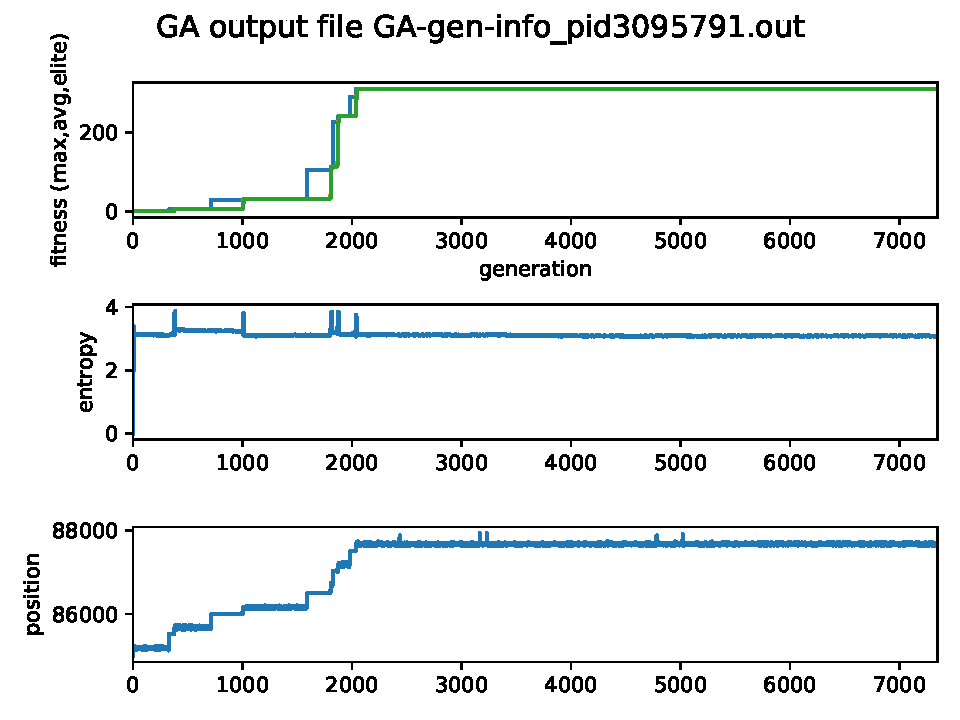
\includegraphics{GA-gen-info_pid3095791.out.pdf}
  }
  \caption{An example of evolution.  The top panel shows fitness as a
    function of generation for a ``$\sin()$ on top of gaussian''
    fitness landscape (see Figure~\ref{fig:fit-func_pid3095791}).  The
    middle panel shows entropy, where you can see that the end point
    of the evolution has a lower entropy than earlier phases.}
  \label{fig:gen-info_pid3095791}
\end{figure}

\begin{figure}[h!]
  \centering
  \resizebox{0.6\linewidth}{!}{%
    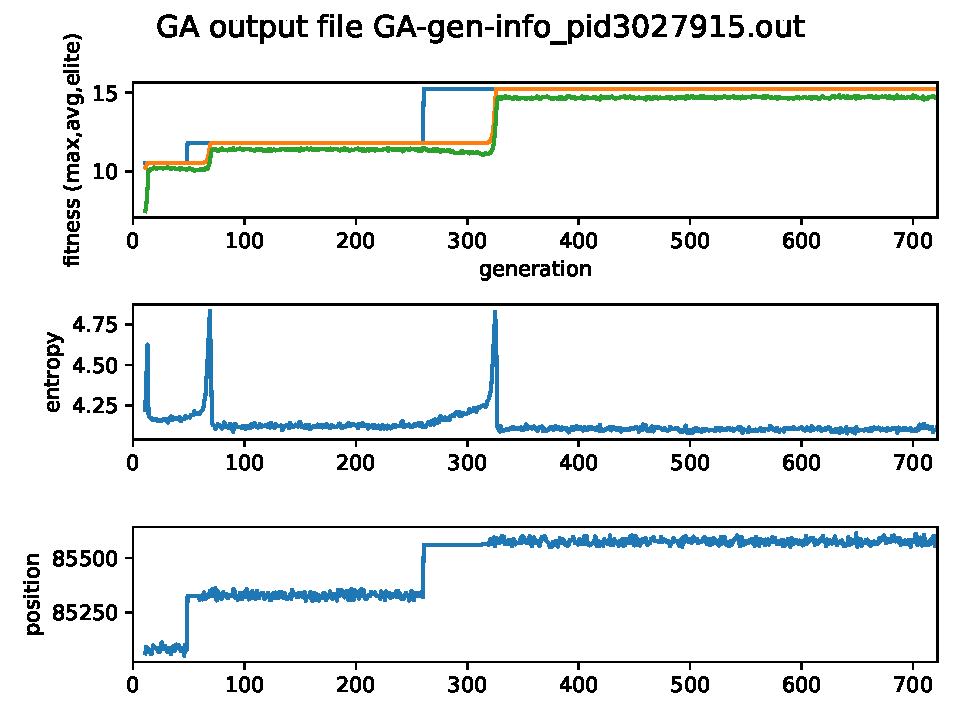
\includegraphics{GA-gen-info_pid3027915.out.pdf}
  }
  \caption{Another example of evolution that shows more clearly how
    the entropy reaches lower pleateaus with increased fitness..}
  \label{fig:gen-info_pid3027915}
\end{figure}




\section{Discussion \& Conclusions}
\label{sec:org7999995}

Entropy rapidly falls as the average fitness makes large steps. This
is because as the x-position value nears the local maxima the
preceding values fall out of the population as the fittest individuals
progress to the next generation. We observed occasional dramatic jumps
in fitness as opposed to a linear development. This is corresponds
with punctuated equilibrium, a theory in evolutionary biology that
evolutionary development is marked by isolated episodes of rapid
speciation between long periods of little or no change (Punctuated
Equilibrium, 2020).

\begin{figure}[h]
	\begin{center}
	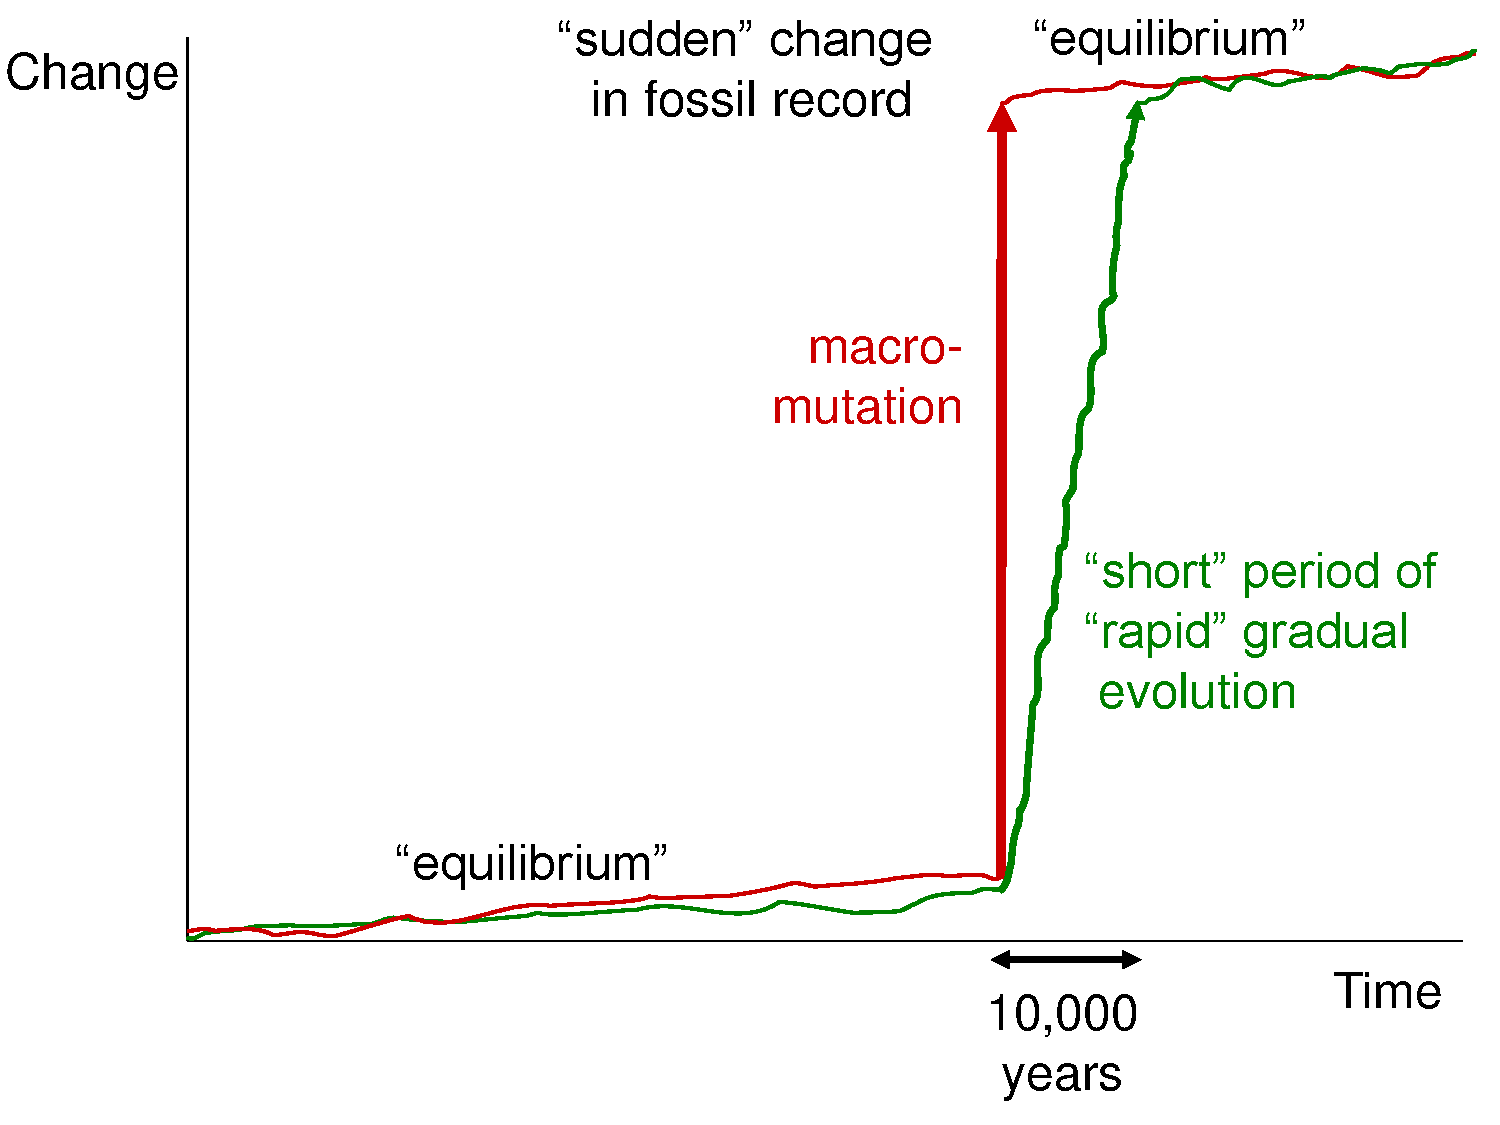
\includegraphics[scale=0.25]{Punctuated_Equilibrium.pdf}
	\caption{ \small Ian Alexander, CC BY-SA 4.0
          <https://creativecommons.org/licenses/by-sa/4.0>, via
          Wikimedia Commons }
\end{center}
\end{figure}

\subsection{What does this mean?}
\label{sec😮rgf7b36ed}

In Figure ~\ref{fig:gen-info_pid3027915} we see how when the average, elite, and max fitness take a
step forward the entropy comes tumbling down. This means that as a
species evolves and better adapts to its environments and beats out
the competition entropy decreases. This does not violate the second
law of thermodynamics because that only applies to an adiabatic
system.

\subsection{Limitations to genetic algorithms}
\label{sec:org148bf83}

There are some limitations to genetic algorithms. For example, one
must have a very clear understanding of the problem, constraints, the
data structure, etc. Additionally, genetic algorithms do not scale
well with complexity -- problems with large numbers of elements often
become exponentially more difficult to compute. There is also the
difficulty of ensuring the algorithm doesn't get stuck on a local
maxima rather than the global one.

\subsection{Future work}
\label{sec:org0f04af1}

Going forward, it could be interesting to optimize a genetic algorithm
from the standpoint of its entropy.

\section{References}
\label{sec:org9dc046e}
\textbf{need to be alphebatized by last name of the first author}\\
\doublespacing

Kinnear, K. E. (1994). In K. E. Kinnear (Ed.), \emph{Advances in
Genetic Programming} (pp. 3-17). Cambridge: MIT Press.

Radcliffe N.J., Surry P.D. (1995) Fundamental limitations on search
algorithms: Evolutionary computing in perspective.  In: van Leeuwen
J. (eds) Computer Science Today. Lecture Notes in Computer Science,
vol 1000. Springer, Berlin, Heidelberg.
$https://doi.org/10.1007/BFb0015249$

Punctuated Equilibrium. (2020). In Oxford Online Dictionary. Retrieved
from $https://www.lexico.com/definition/punctuated_equilibrium$

\end{document}
